\chapter{Implementation Details}

\section{Document management}

The current section consists of three parts:

\begin{itemize}
\item The first explains the prototype we wrote.
\item The second details implementation challenges when realizing the designed extension and using external libraries.
\item The third shows changes in the extension visible from a user's point of view, with screenshots.
\end{itemize}

\subsection{The prototype}

As mentioned already, the SharePoint protocol has a brief reference
documentation on MSDN, but that is not enough to create an open-source
implementation of the protocol. To solve that issue, we used two virtual
machines:

\begin{itemize}
\item One running Microsoft SharePoint 2007.
\item The other running Microsoft Office 2007.
\end{itemize}

Finally we used Wireshark\cite{wireshark} to monitor the network traffic
between the two virtual machines to reverse engineer the details of the
protocol missing from the reference documentation.

Trying to reimplement the protocol directly in the LibreOffice extension would
make development slow, partly because that would mean solving UNO interfacing
issues and Java design decisions at the same time, partly because we needed a
simple script to demonstrate how the protocol works, where Java may not be the
best language to use. As a consequence, we decided to write a command-line
prototype in Python, a popular scripting language, and once that was ready and
worked, we ported the logic of the prototype to Java.

The prototype had commands (open, save, delete, etc.) to test each feature
individually.  This covered the functionality outlined in the \emph{Background}
chapter, except that folder / document listing is implicit here: the open and
save-as operation invoked that, but it had no explicit command assigned.

The prototype also had two switches to test the implementation on both
SharePoint and Alfresco automatically. This was critical, so that when we fixed
something to work with Alfresco, we could quickly test we did not break
anything in SharePoint.

Once the used protocol -- at least the parts required by our use-cases -- was
clear, we could begin writing the LibreOffice extension.

\subsection{External libraries}

It was obvious that doing HTTP communication with NTLM authentication is an
already solved problem, but we needed to decide which library to use. Given that
OPAL already used Apache \emph{commons-httpclient}\cite{httpclient} 3.x for
HTTP communication, that was an option. Unfortunately that version does not support NTLM, so we used
Apache \emph{httpcomponents}\cite{httpcomponents}, which is the successor of
the previous library (starting with version 4.x). The two version series have
different APIs, so it was possible to temporarily use both in parallel, and migrating code
incrementally.

Once we had \emph{httpcomponents}, we still needed to write detection code that
decided what to request from \emph{httpcomponents}: Basic or NTLM
authentication.

An other interesting issue was to parse the response received after sending
Vermeer RPC requests to the server. The result is valid HTML, but not XHTML.
For example, part of the response is:

\begin{lstlisting}
<html><head><title>vermeer RPC packet</title></head>
<body>
...
<li>vti_timecreated
<li>TR|27 Feb 2011 19:07:25 +0000
<li>vti_timelastmodified
<li>TR|11 Mar 2011 16:39:35 +0000
<li>vti_timelastwritten
<li>TR|11 Mar 2011 16:39:35 +0000
...
</body>
</html>\end{lstlisting}

That means a simple XML parser was not enough to extract the needed values from
this response. To solve this issue, we used TagSoup\cite{tagsoup}, which is a
SAX parser, accepting plain old HTML input.

\subsection{User interface}

Once the Sharpeoint Library was ready, we updated the user interface to use the
SharePoint library for communication. We also had to extend the dialogs to allow
a few more features. Namely:

\begin{itemize}
\item Create and delete document workspaces.
\item Delete documents.
\item Delete and restore versions.
\item When saving a document, allow: minor change with a comment and overwrite of a previous version.
\end{itemize}

For example, creating a new document workspace is implemented as can be seen on
figure~\ref{fig:implementation-createdws}.

\begin{figure}[H]
\centering
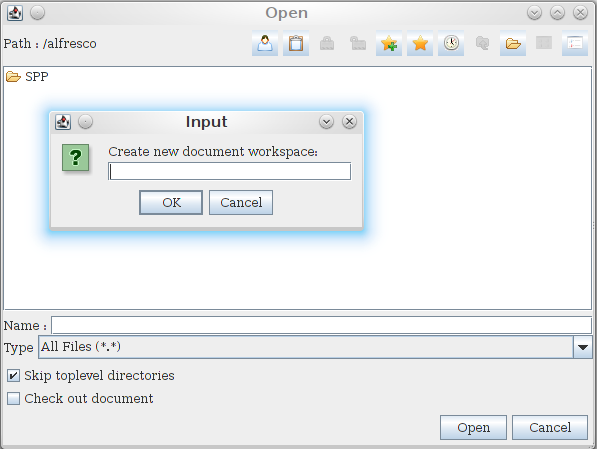
\includegraphics[width=250px,keepaspectratio]{implementation-createdws.png}
\caption{Implementation of creating a document workspace}
\label{fig:implementation-createdws}
\end{figure}

Earlier it was possible to only view older versions, the new \emph{Versions}
dialog now allows a user to delete and restore versions as well (as detailed
above in table~\ref{tab:background-comparison}, deleting versions does not work
with Alfresco, due to the shortcomings of their SharePoint implementation), see
figure~\ref{fig:implementation-versiondialog}.

\begin{figure}[H]
\centering
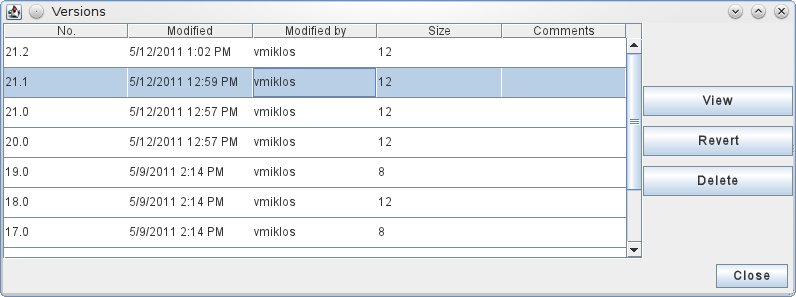
\includegraphics[width=400px,keepaspectratio]{implementation-versiondialog.png}
\caption{Implementation of version restore and delete}
\label{fig:implementation-versiondialog}
\end{figure}

\subsection{Exception handling}

The last challenge was the localization of error messages in BASIC. The
language does not support any kind of localization. What it supports is the
following technique:

\begin{lstlisting}
Sub openVersion
...
        On Error GoTo errSpDoc
        oVersion.execute()
        Exit Sub

        errSpDoc:
                MsgBox(oVersion.ErrorReason)
                Exit Sub
End Sub
\end{lstlisting}

The \emph{On Error} part can hide any kind of exception thrown by Java, and as
long as the Java side calls \emph{setErrorReason()} on the
\emph{SharepointVersionsImpl} object before throwing an exception, the user gets
a friendly error message, which is even localized.

\section{Workflows}

The implementation of workflow integration had multiple interesting challenges:

\begin{itemize}
\item adding support for the authentication method jBPM uses
\item handling data received in responses from jBPM
\item error handling in multiple levels
\end{itemize}

\subsection{Authentication}

jBPM uses form-based authentication. That means that in case the user is not
yet logged in, she is redirected to a login form, where the user name and
password should be submitted. The \emph{httpcomponents} package provides a
dedicated \emph{UrlEncodedFormEntity} class for this purpose:

\begin{itemize}
\item Fields in the form should be collected to a \emph{NameValuePair} list;
\item Once the list is ready, the entity generator class can produce the
necessary payload for the HTTP request, using the
\texttt{application/x-www-form-urlencoded} MIME type\cite{form-encoding}.
\end{itemize}

There are two problems here:

\begin{itemize}
\item The user interface expects a stateful connection here, while HTTP is stateless.
\item The password is sent without encryption.
\end{itemize}

The first problem can be solved multiple ways. First, the workflow handler can
remember the credentials passed from the user interface, hiding the repeated
login procedure from the user. Alternatively, in this case jBPM handles
sessions, so receiving and sending back cookies avoids multiple logins as well.

The problem of clear-text passwords sent over the network can be solved at an
application server level, in case HTTPS is used.

From a user experience point of view an additional problem is the confusing
connection dialog that asks for multiple user names and passwords. Given that
we are integrating the document management and the workflow system, we can
expect that the same credentials are used by the same users to access these
servers. As a result, the user interface asks for a single login and password,
the Java implementation does two logins in practice, though. The user interface
signals an error in case any of these logins failed.

\subsection{JSON handling}

Most responses received from the jBPM server are JavaScript Object Notation
(JSON) strings. The interested reader can look into the
specification\cite{json}, all we need to know about it here is that it can
represent a set of Java objects, allowing references between them.

Once entity classes are available (as described in the \emph{Design} chapter),
the Gson library\cite{gson} can be used to parse those strings to entity class
instances.

The benefits of using Gson over other implementations (like
\emph{org.json}\cite{org-json}):

\begin{itemize}
\item it requires no pollution of the entity classes regarding JSON (i.e. no \emph{toJson()} methods are necessary)
\item when a default constructor is not available for an entity class, it supports the registration of instance creators for such types
\end{itemize}

It uses reflection to access fields, so the usual implementation can
be used: the fields themselves are private and public getter/setter methods are
provided. Also, the parser is quite liberal about entity classes, in case a
field is part of the JSON string but the associated Java class does not have
such a field, it is simply ignored. That helps our extension to be compatible
with future jBPM server versions.

A pitfall during the implementation was that the usage of generic types is
mandatory when using references between the classes:

\begin{itemize}
\item In case a generalized collection is used as a field type, Gson can extract the type information of the referenced objects from the field type, and instantiate the correct class.
\item Otherwise, there is no way to guess the type of the referenced instance, so a parse exception is thrown.
\end{itemize}

\subsection{User interface}

\begin{figure}[H]
\centering
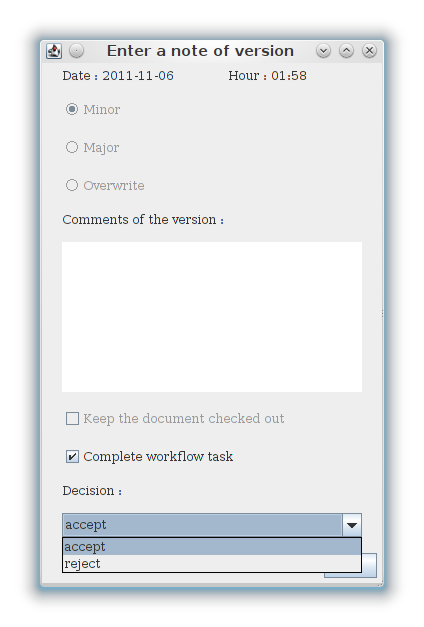
\includegraphics[width=200px,keepaspectratio]{implementation-decision.png}
\caption{Implementation of making a business decision when completing a human task}
\label{fig:implementation-decision}
\end{figure}

\begin{figure}[H]
\centering
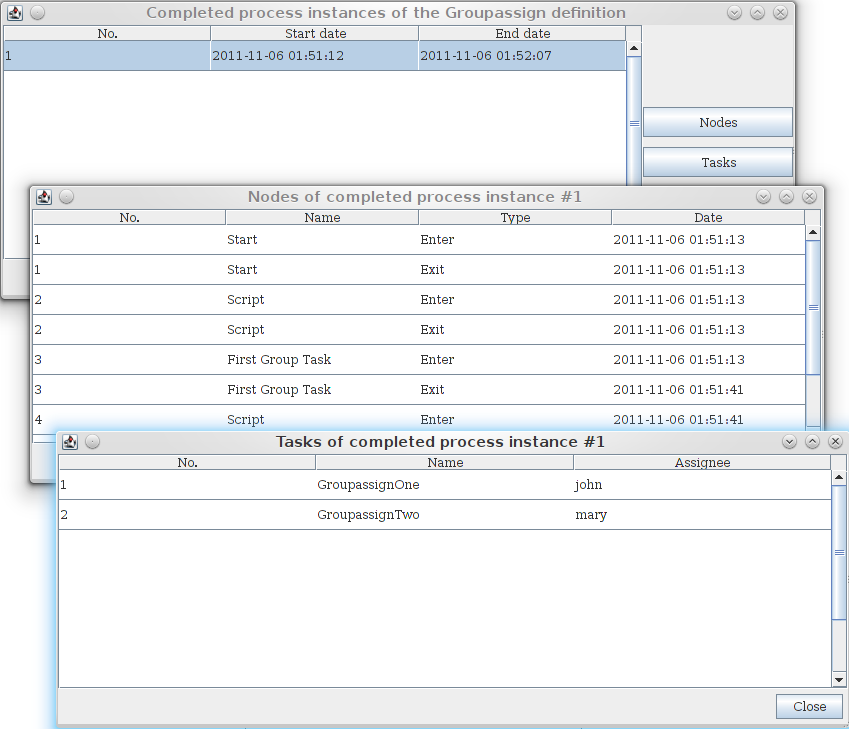
\includegraphics[width=400px,keepaspectratio]{implementation-auditlog.png}
\caption{Implementation of the audit log: process instances, node instances and users performing human tasks}
\label{fig:implementation-auditlog}
\end{figure}

\subsection{Error handling}
